

\chapter*{SVM}
Pour la reconnaissance du geste dans ce challenge on pouvait choisir entre 3 différents algorithmes de machine learning. J'ai choisi SVM parce que c'était l'algorithme que j'avais compris le plus. j'avait le dut avec choiri ANN mais a été choisì par mon collègue Marco. HMM il parait entre le plus adapté par la structure des données à traiter mais il est plus compliqué a mettre en place ainsi.

\section*{Pretraitement}
Dans la phase de pretraitement il a été effectué une modification initiale de données brute pour le mieux visualiser et pour le rendre plus lisible.
 Pour ce faire pn a créee de Histogramme pour chaque caractéristique pour visualiser mieux dans quelle "range" de valeur était présent pour chaque geste. 

Dans l'image \ref{fig:prehist} on peut voire trois exemple d'un histogramme fait accélération de la main dans l'axe des Y.

On peut voire que le range de valeur va entre -1  jusqu'à 1 pour la majorité des points.
\begin{figure}[h]
  \centering
    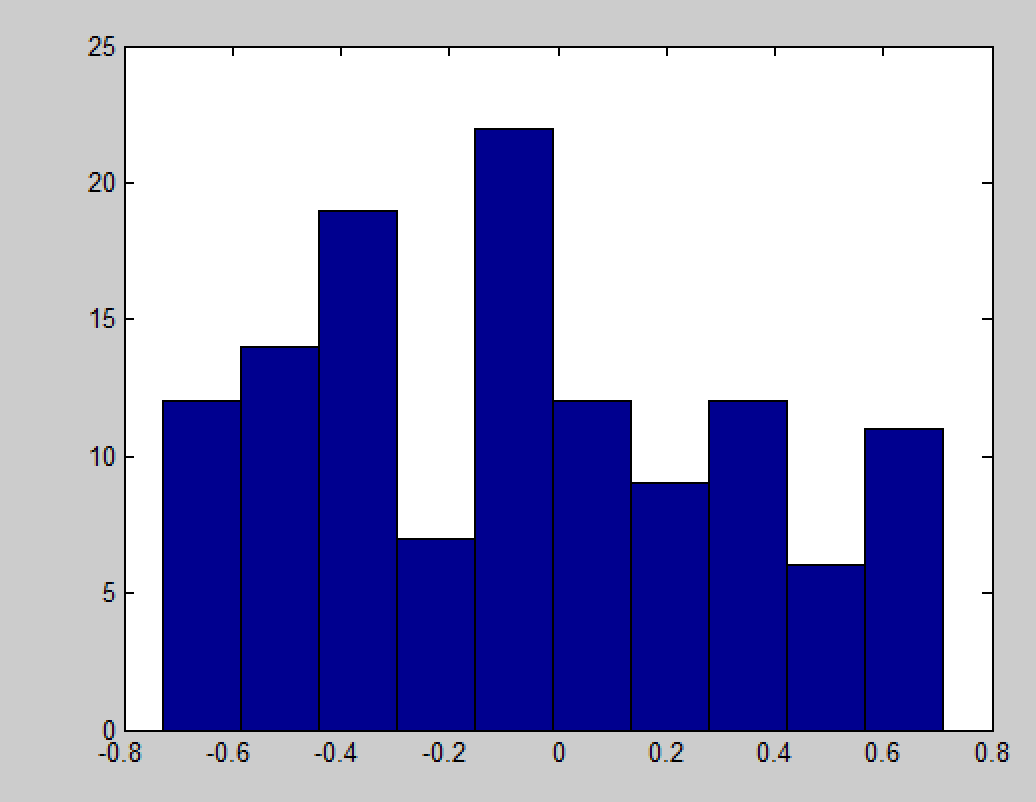
\includegraphics[width=0.5\linewidth]{img/pretraitement/hist10.png}
  \caption{histogramme du signal AccX de la class 1}
  \label{fig:prehist}
\end{figure}

En addition â la lisibilité du signal un histogramme peut etre tres utile pour reppresenter un signal continue en un unique vecteur de valeur pour entrainer un SVM. 
En effet SVM veut en entrée une matrice ou chaque ligne corrispond a un classe complete. Il a follu donc parcourrir toutes les observation d'une classe pour pouvoire creer un histogramme et le donner en entree à notre SVM.




\section*{Extraction des caractéristiques}
Dans cette phase on a pu utiliser les histogramme fait dans le pretraitement pour mieux comprendre les caracteristiques. Il a été effectué un comparaison entre plusieur histogramme fait sur lem'eme signal mais avec de classe differents. Dans l'image \ref{fig:histogram-pre} on peut voire que l'histogramme du signal AccX est assais different pour el trois classe mise en evidence.

Ce signal peurra donc entre un bon candidat pour differentier les differents classes et pour entrainernotre modele. 


\begin{figure}[h!]
    \centering
    \begin{tabular}{cccc}
      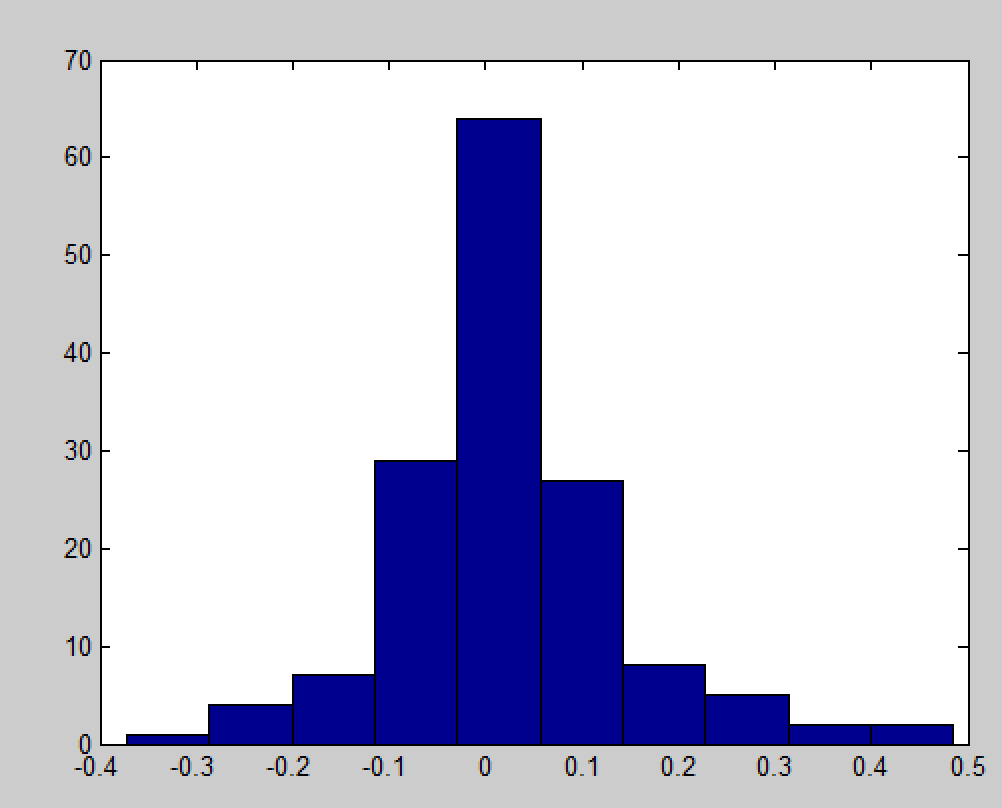
\includegraphics[width=.30\linewidth]{img/pretraitement/hist0.png} &
      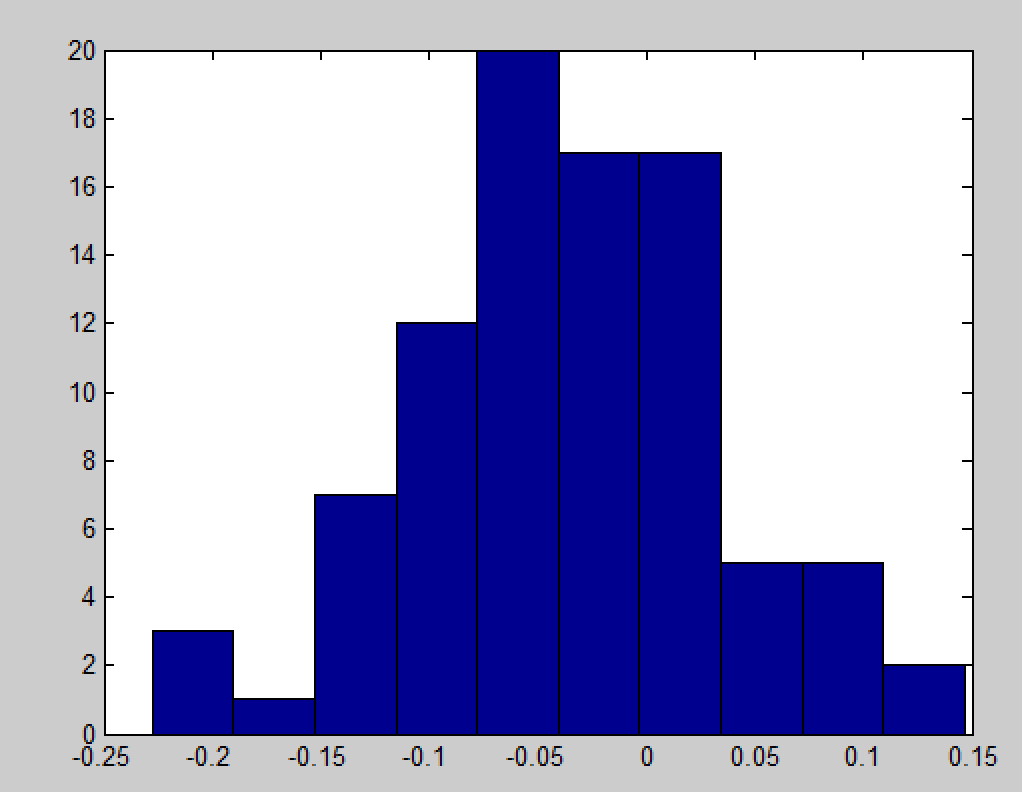
\includegraphics[width=.30\linewidth]{img/pretraitement/hist1.png} &
      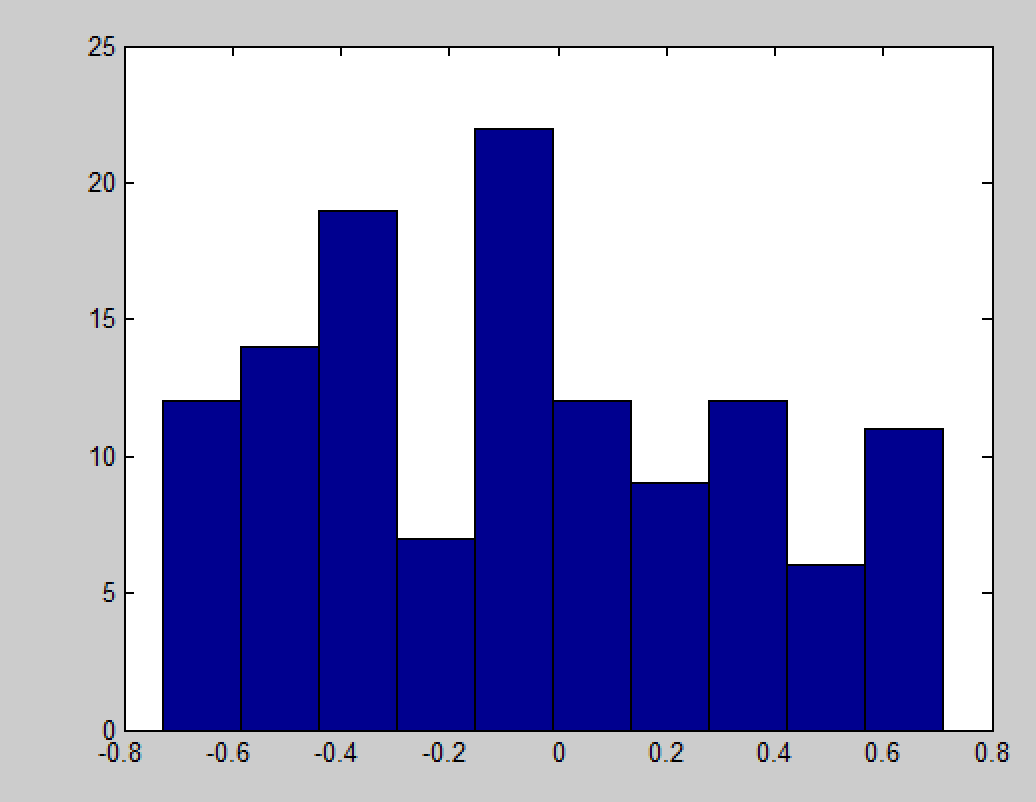
\includegraphics[width=.30\linewidth]{img/pretraitement/hist10.png} \\
      (a) & (b) & (c)\\
    \end{tabular}
    \caption{AccX pour le classe (a) 0 (b) 1 (c) 10
    \label{fig:histogram-pre}}
\end{figure}


En plus des l'"AccX" il à été utilise le "AccY", "AccZ" de la main et le "AccX","Z" du bracelet ainsi que le signal "Pinch" de la main.

Ces differents histogrammes  des carcacteristiques a été mis ensemble pour donner un unique vecteru des caracteristique. 

Un visualisation des histogramme mis ensemble pour quatre differents classe est montré dans l'image \ref{fig:histvector}. Dans cette figure sont montré toutes les occurence de chaque classe.

\begin{figure}[h]
  \centering
    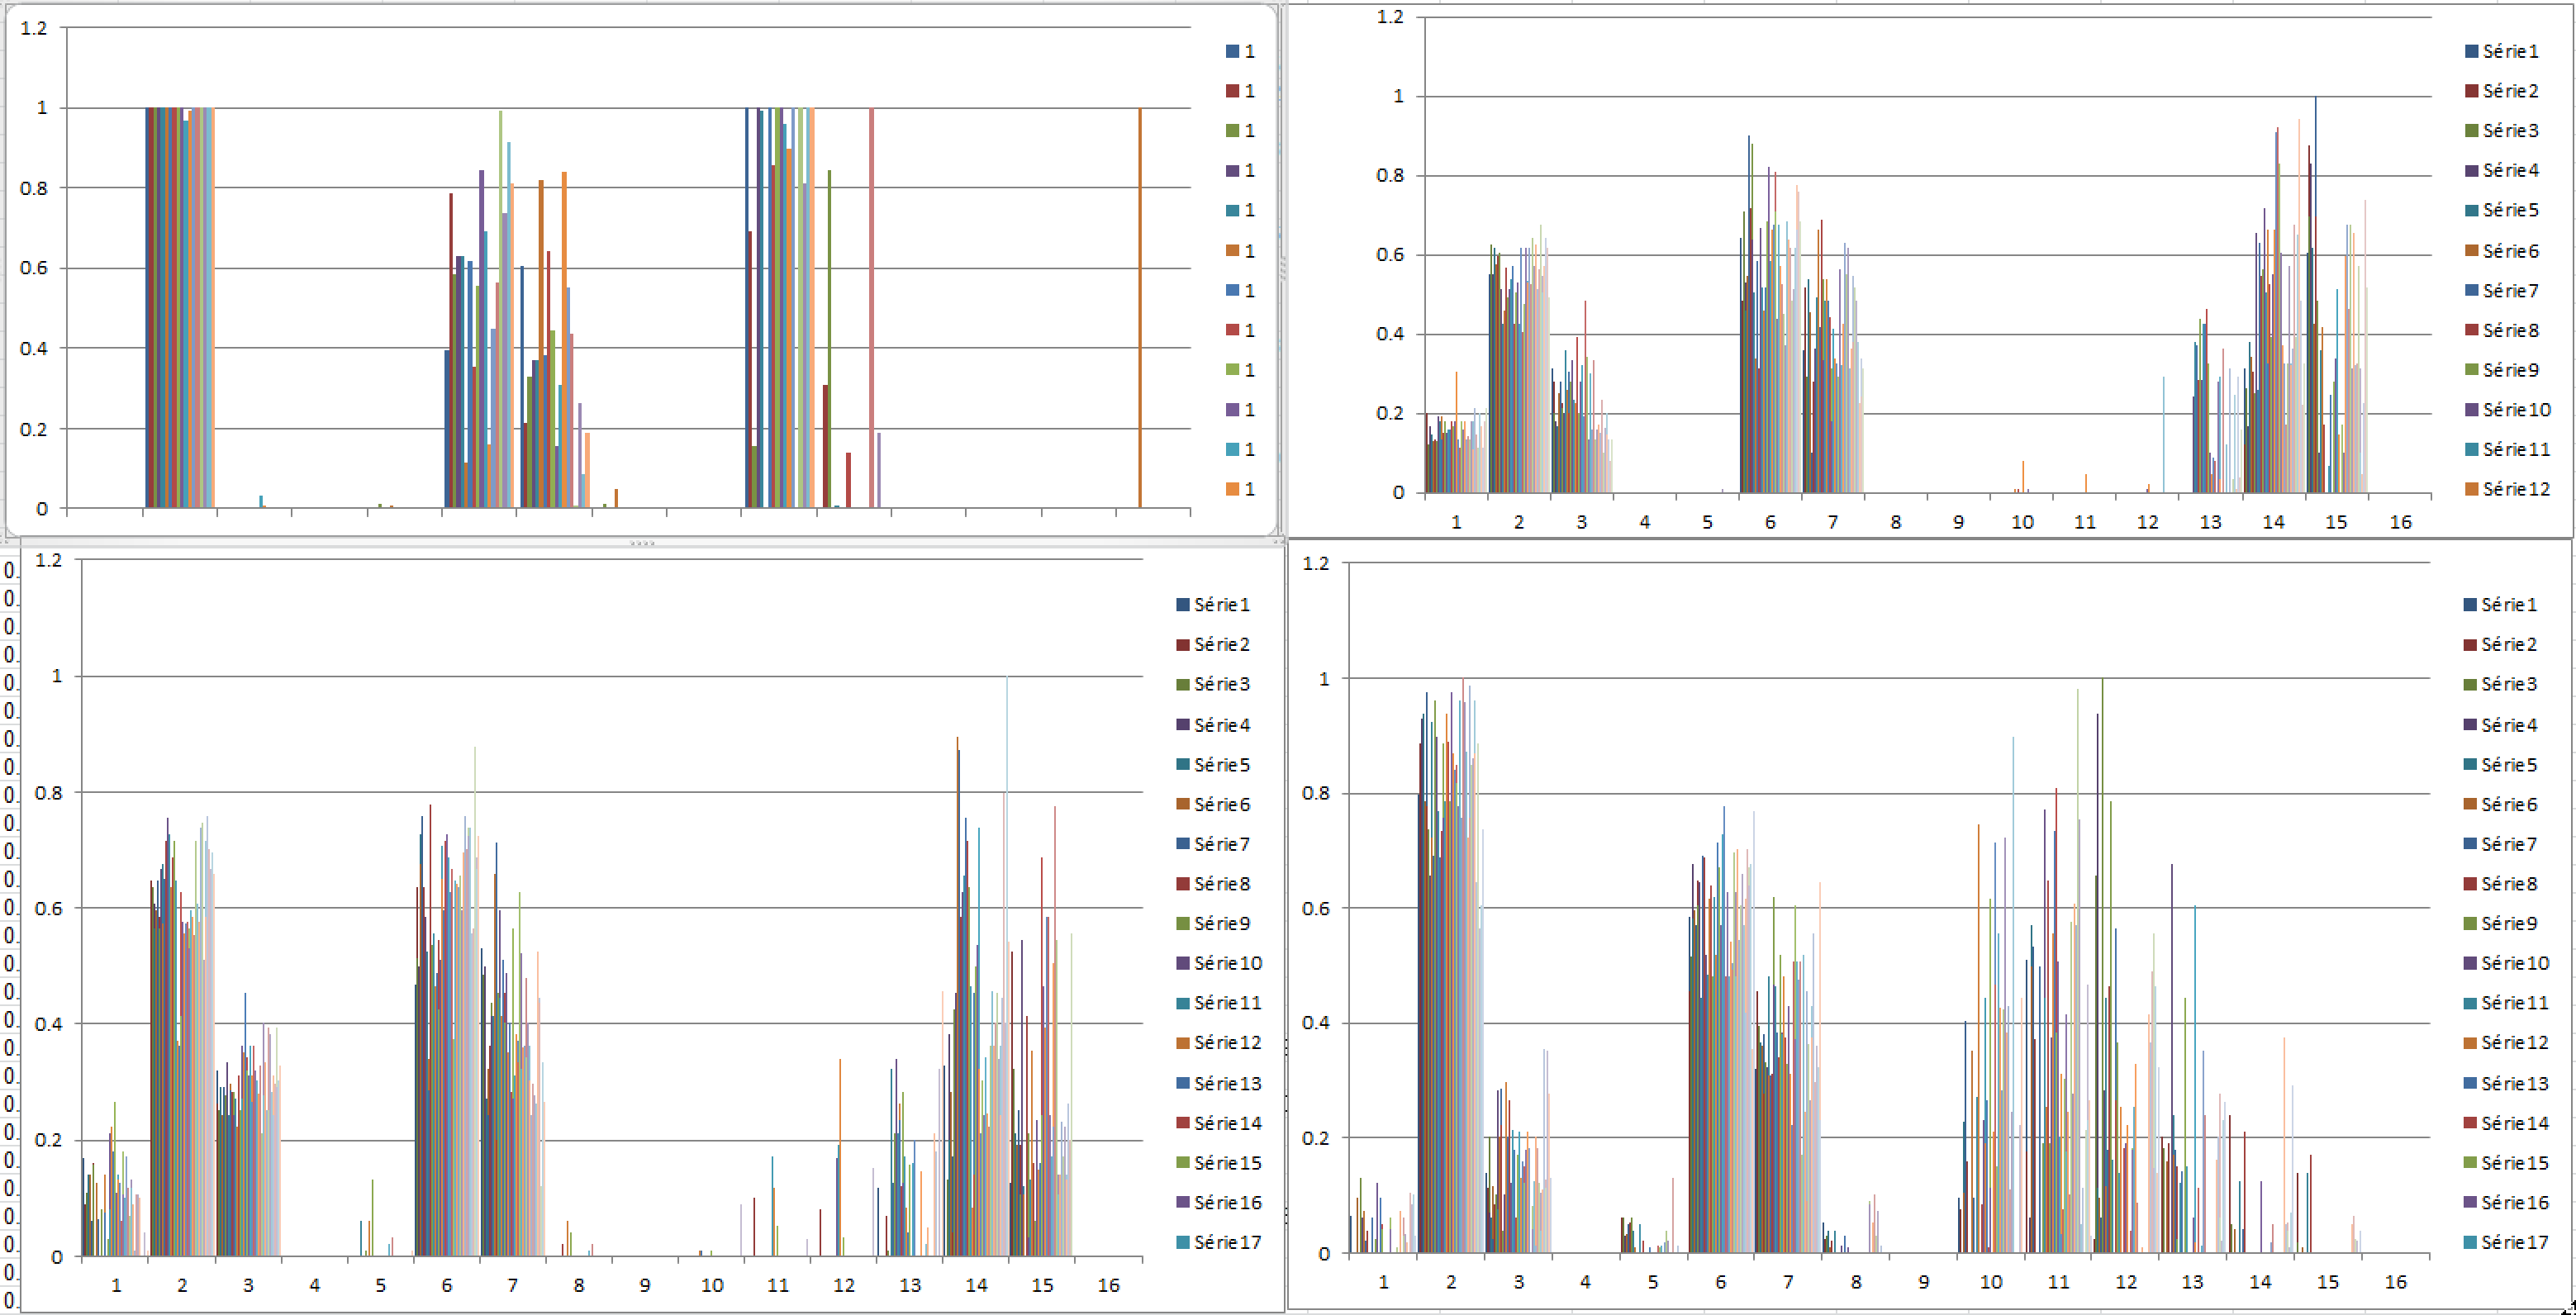
\includegraphics[width=1\linewidth]{img/extraction/vector-hist.png}
  \caption{Group of histogramme for a unique vector for four classes}
  \label{fig:histvector}
\end{figure}

O peut voire de cette figure que la forme des histogrammes pour un geste est presque identique pour toutes le soccurence.Par contre il est assas different pour un outre geste.

\section*{Entrainement}
Pour entrainer le SVM on a besoin d'une matrice ou chaque ligne reresent un geste et chaque colonne une feature. Dans notre cas pour chaque histogramme on a plus ou moin 10 feature qui sont reppresenté par un nombre de 0 a 1. 

\begin{lstlisting}[language=python]
    for i=1:NUM_CLASSES %Train model for all classes
        label=(Y==i); %Convert multi class to double class 1 or 0
        svmStructs(i) = svmtrain(X,label,'kernel_function','polynomial');
    end  %code insipred to multiclass svm
\end{lstlisting}

\section*{Évaluation}
L'evaluation des données de tests a été effectué en utilisant le modele crée durant l'entrainement. Pour utilise un SVM binaire pour reconaitre plusieurs classe on fait un evaluation de chaque modele créee lors le l'entrainement avec le geste du test. La classe de test sera identifié quand un des ces modeles respond positivement.

le diagramme \ref{fig:models-svm} montre en maniere schematique comment ce algorithme fonctionne, On peut voir que chaque entree verra evelué par chaque modee SVM jusqu'a un modee le reconait.

Le probleme de cette methode est que si aucun des modele reconnait la classe d'un instance de tests un valeur par default lui sera attributé dans notre case la classe 10.

Cela ça peut devenir un problem quand le geste seront beaucoup et similaire entre eux. Un manierepour ammeliorer ça peurra entre d'attribuer un score à chaque evalaution de classe et au final choisi celle avec le plus grand score.


\begin{figure}[h]
  \centering
    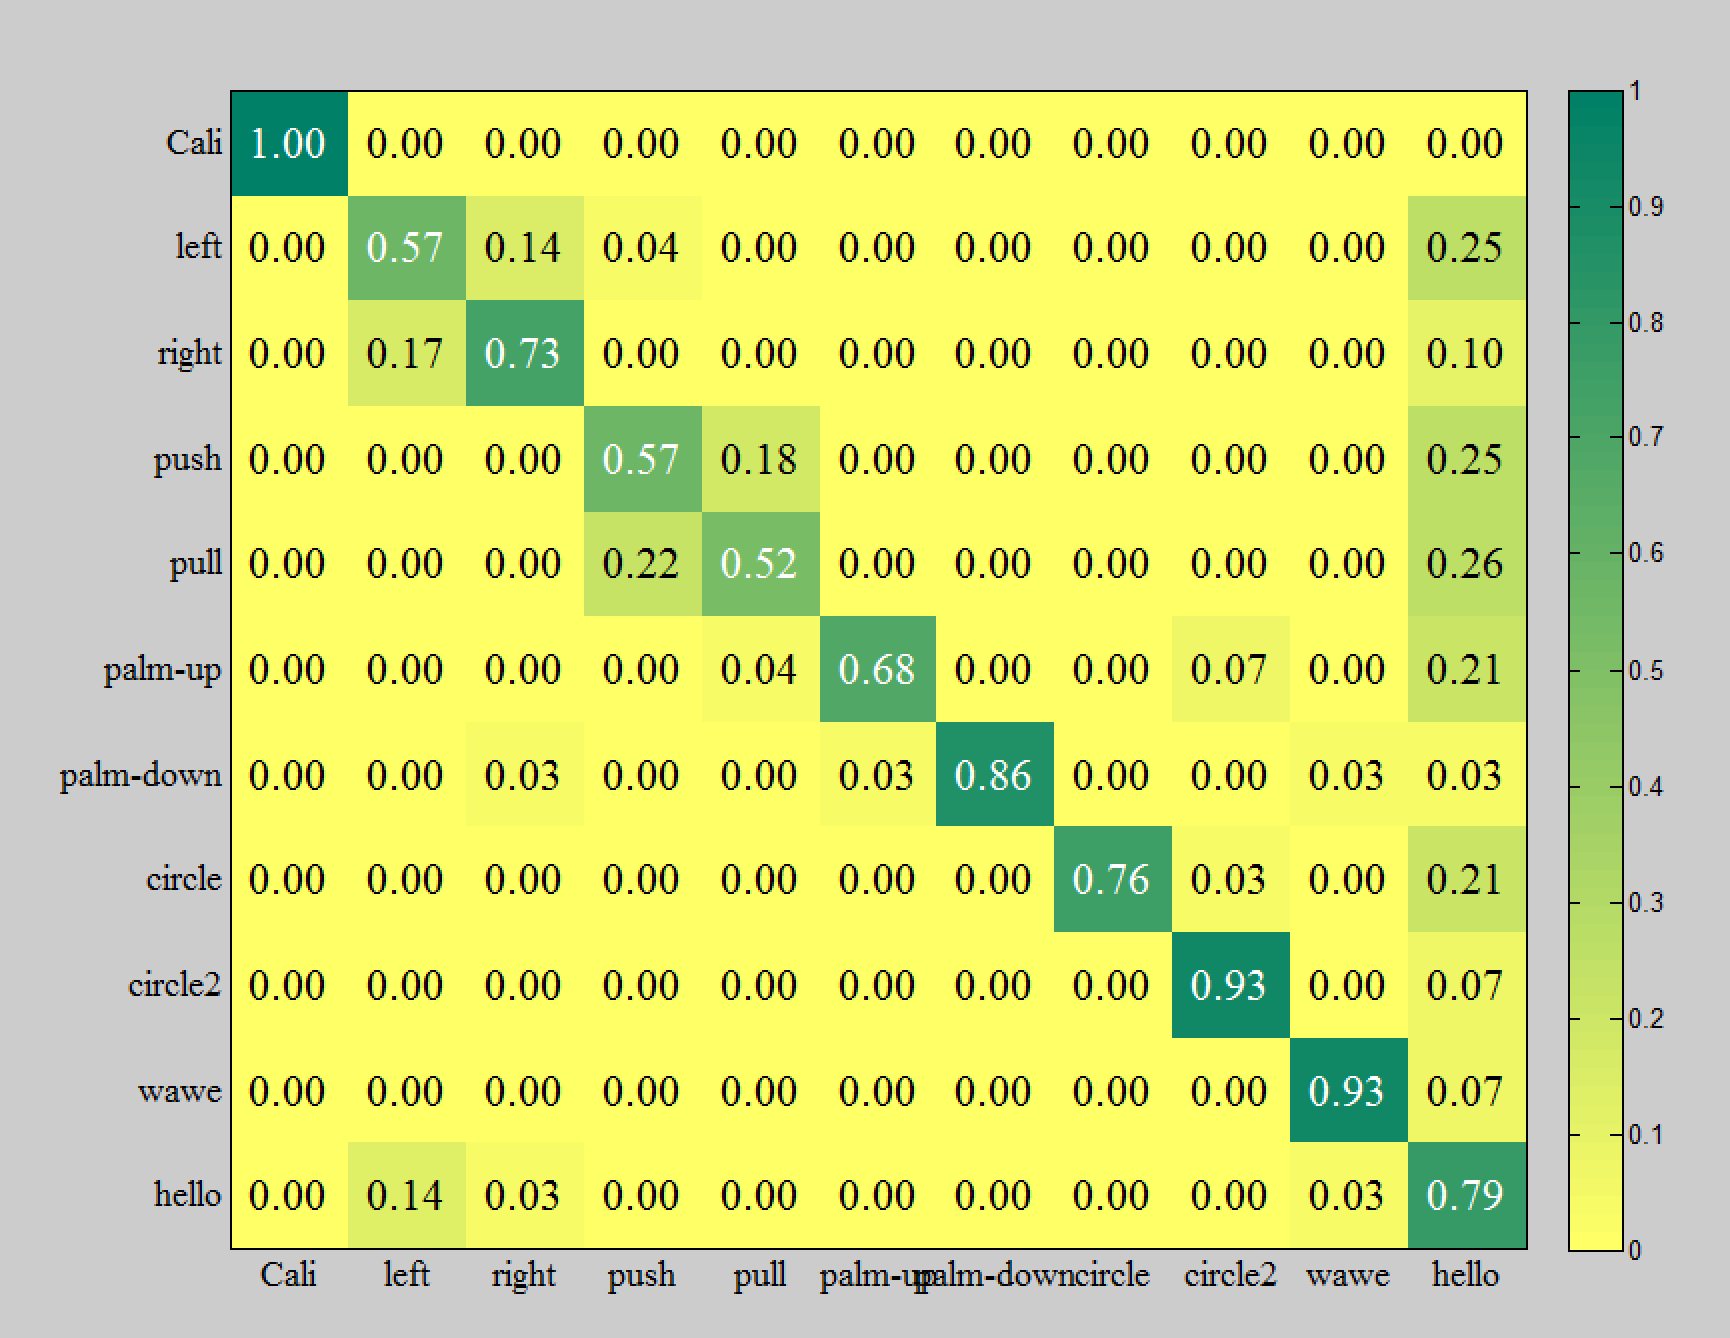
\includegraphics[width=0.7\linewidth]{img/evaluation/confusion.png}
  \caption{Group of histogramme for a unique vector for four classes}
  \label{fig:histvector}
\end{figure}


\section*{Résultats obtenu}
Dans la matrce de confusion obtenu  depuis l'evaluation du set de test on petu voireque le classe sont assais bien classifier parce que sont distrubue pour la plupart sur la diagonale.

Par contre il a encore quelque geste que l'algorithme l'echange avec un outre geste similaire ou qu'il a encore beaucoup d'erreur de reconnaissance. On voit par exemplque que l'algorithme `un certen difficulté a 

\section*{Problèmes rencontrées}
-dsvm
-fitcecoc


\section*{Perspectives et améliorations}


% Code integration example
%\begin{lstlisting}[language=bash]
%  sudo apt-get update
%  sudo apt-get install drupal7
%\end{lstlisting}

% Image integration example
%\begin{figure}[h]
%  \centering
%    \includegraphics[width=1\linewidth]{img/drupalFirstPage.png}
%  \caption{Page d'accueil du site créé avec Drupal sur une instance EC2}
%  \label{drupalfirstpage}
%\end{figure}

% Image side-by-side
%\begin{figure}[h!]
%    \centering
%    \begin{tabular}{cccc}
%      \includegraphics[width=.14\linewidth]{randomTree_n5.png} &
%      \includegraphics[width=.22\linewidth]{randomTree_n10.png} &
%      \includegraphics[width=.22\linewidth]{randomTree_n15.png} \\
%      (a) & (b) & (c)\\
%    \end{tabular}
%    \caption{Arbres aléatoires où (a) n=5 (b) n=10 (c) n=15
%    \label{randomTrees}}
%\end{figure}
